\documentclass[DIV=calc, paper=a4, fontsize=11pt]{scrartcl}


\usepackage{makeidx}
\usepackage{graphicx}
\usepackage{flushend}

\usepackage{lmodern}
\usepackage[left=1.5cm,right=1.5cm,top=2.5cm,bottom=2cm]{geometry}
\usepackage{float}		
\bibliographystyle{plain} 
\pagestyle{plain} 
\pagenumbering{arabic}
\usepackage{fancyhdr} 	
\usepackage{siunitx}


\usepackage[T1]{fontenc}
\usepackage[utf8]{inputenc}
\usepackage[spanish]{babel}
\usepackage{hyperref}
\usepackage{graphicx}

\usepackage{lipsum}
\usepackage[protrusion=true,expansion=true]{microtype}
\usepackage{amsmath,amsfonts,amsthm}
\usepackage[svgnames]{xcolor}
\usepackage[svgnames]{xcolor}
\usepackage{booktabs}
\usepackage{fix-cm}
\usepackage{multicol}
\newenvironment{Figura}
  {\par\medskip\noindent\minipage{\linewidth}}
  {\endminipage\par\medskip}

\usepackage{sectsty}
\allsectionsfont{\usefont{OT1}{phv}{b}{n}}

\usepackage{fancyhdr}
\pagestyle{fancy}
\usepackage{lastpage}

\lhead{}
\chead{}
\rhead{}

\lfoot{}
\cfoot{}
\rfoot{\footnotesize Page \thepage\ of \pageref{LastPage}}

\renewcommand{\headrulewidth}{0.0pt}
\renewcommand{\footrulewidth}{0.4pt}

\usepackage{lettrine}
\newcommand{\initial}[1]{\lettrine[lines=3,lhang=0.3,nindent=0em]{
\color{DarkGoldenrod}{\textsf{#1}}}{}}

\usepackage{titling}

\newcommand{\HorRule}{\color{DarkGoldenrod} \rule{\linewidth}{1pt}}

\pretitle{\vspace{-120pt} \begin{flushleft} \HorRule \fontsize{22}{35} \usefont{OT1}{phv}{b}{n} \color{DarkRed} \selectfont}

\title{Calculo de la Densidad\\ %Aquí va el nombre de la práctica 
Práctica 4} %Numero de la práctica 

\posttitle{\par\end{flushleft}\vskip 0.5em}

\preauthor{\begin{flushleft}\large \lineskip 0.5em \usefont{OT1}{phv}{b}{sl} \color{DarkRed}}

\author{Misael Iván Macías Márquez\\
misaelmacias@ciencias.unam.mx}

\postauthor{\footnotesize \usefont{OT1}{phv}{m}{sl} \color{Black}

\vspace*{0.1cm} Facultad de Ciencias, UNAM

\par\end{flushleft}\HorRule}

\date{Martes 5 de Abril de 2022\\Semestre 2022-2}


\begin{document}

\maketitle


\begin{abstract}
\textbf{Resumen:} Se determinaron las densidades de distintos líquidos y monedas tomando varias mediciones de masa y volumen para después linealizar y ajustar por mínimos cuadrados, los resultados se compararon con las densidades reportadas en distintas fuentes de cada material usado los resultados aunque no muy buenos se pueden considerar satisfactorios para haberse realizado con material casero, también se comparó la densidad y temperatura del agua para diferentes cantidades de sal, la temperatura respecto a la densidad parece seguir la misma tendencia para cada cantidad de sal solo que conforme esta aumenta la gráfica se desplaza hacia arriba.
\end{abstract}

\begin{multicols}{2}




\section*{Introducción}

La densidad $\rho$ para un objeto homogéneo de masa $m$ y volumen $V$ es una cantidad escalar que se define como:

\begin{equation}
    \rho = \frac{m}{V}
\end{equation}

o bien [2]:

\begin{equation}
    m = \rho V
\end{equation}

La densidad de un material en general depende de factores ambientales, incluyendo la presión y la temperatura. En los líquidos y en los sólidos, la variación de la densidad es muy pequeña dentro de  intervalos grandes de presión y de temperatura, y en muchas aplicaciones podemos considerar a la densidad como una constante[2].





\section*{Desarrollo experimental}

\begin{Figura}
\centering
    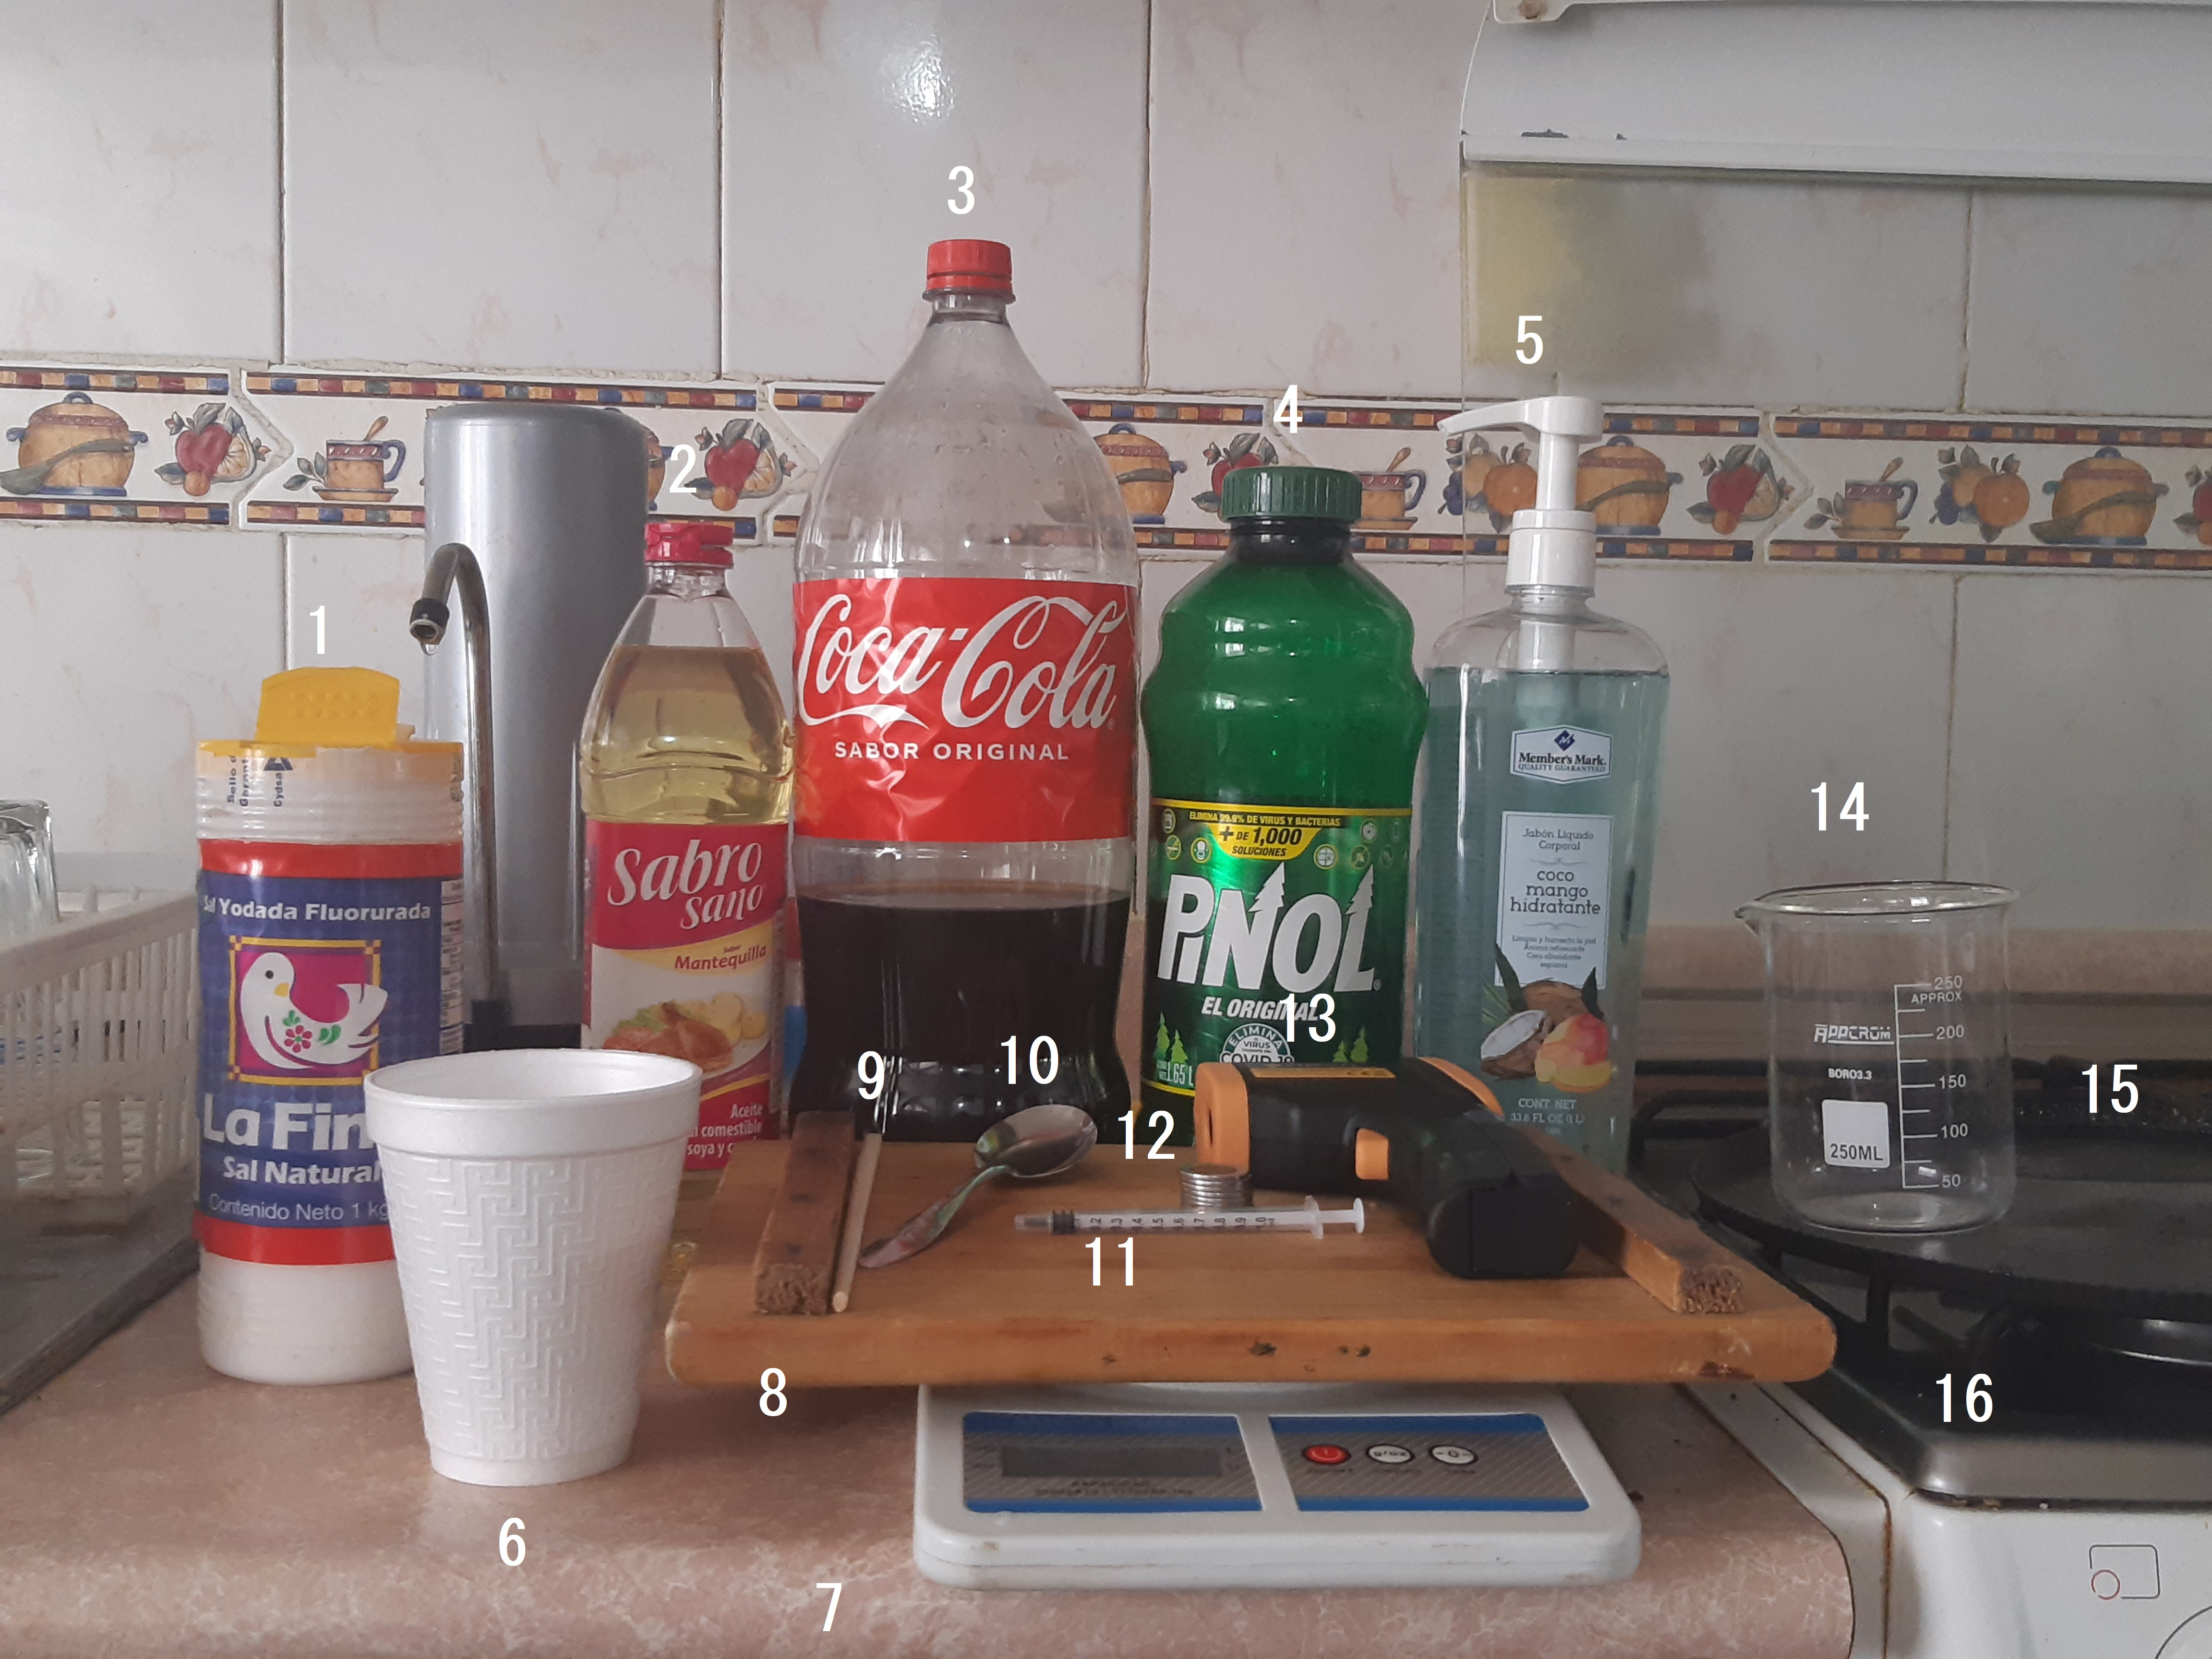
\includegraphics[width=0.8\textwidth]{20220302_135437.jpg}
    \captionof{figure}{Material y arreglo experimental: (1) sal, (2) aceite, (3) refresco, (4) detergente liquido, (5) jabón liquido, (6) vaso de unicel, (7) báscula digital, (8) tabla de madera, (9) agitador, (10) cuchara, (11) jeringa, (12) monedas de 1 peso, (13) termómetro digital, (14) vaso de precipitados, (15) comal, (16) estufa}
    \label{fig}
\end{Figura}

\subsection*{PARTE I}

Con ayuda de la bascula digital se midió la masa $m$ de una moneda para posteriormente agregar otra moneda y seguir así hasta tener la masa de las 10 monedas juntas, después con la cinta métrica se midió el radio $r$ de una moneda y su grosor $d$.

Para las densidades de los líquidos se usó un vaso de precipitados de 250mL para medir 9 diferentes volúmenes, para el décimo volumen se utilizo una taza medidora extra. Las masas de los líquidos fueron medidos con la bascula digital y restando el peso del envace(s) que lo contenía.

\subsection*{PARTE II}

Con el vaso de precipitados se midieron 200 mL de agua para después medir su peso y temperatura, ya con esto se procedió a calentar el agua hasta los 40 $C$ colocando el vaso de precipitados en el comal sobre una hornilla encendida después de medir su masa y volumen se repitió esto para el resto de temperaturas y salinidades, para medir la diferencia de volumen se utilizo una jeringa de 1mL y un vaso de  unicel para colocar el excedente o de donde sacar lo faltante de los 200 mL 




\section*{Resultados y Análisis}



\subsection*{PARTE I}
Usando la ecuación 2 y linealizando las mediciones se obtienen las densidades de cada liquido y monedas como las pendientes ajustadas por el método de mínimos cuadrados. La incertidumbre de estas pendientes se obtiene de la misma función usada para ajustar por mínimos cuadrados.

La densidad resultante para las monedas de un peso es:

\begin{equation*}
    m_1 = 5.894 \pm 0.045 \frac{g}{cm^3}
\end{equation*}

y la densidad de las monedas de un peso es $5.702 \frac{g}{cm^3}$$\footnote{https://www.banxico.org.mx/billetes-y-monedas/moneda-1-peso-familia-c-circu.html}$.

\begin{Figura}
\centering
    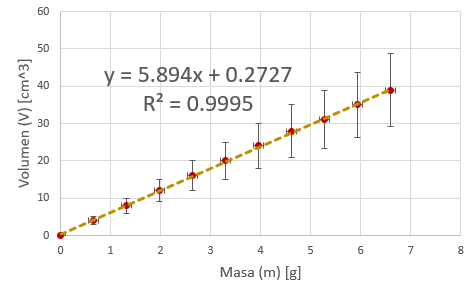
\includegraphics[width=0.8\textwidth]{grafica monedas.PNG}
    \captionof{figure}{Gráfica del ajuste por mínimos cuadrados
para los datos de las monedas linealizados según la
ecuación 2.}
    \label{fig}
\end{Figura}

La densidad resultante para el agua es:

\begin{equation*}
    m_2 = 0.980 \pm 0.017 \frac{g}{cm^3}
\end{equation*}

y la densidad del agua es de $0,998 \frac{g}{cm^3}\footnote{https://www.iagua.es/respuestas/cual-es-densidad-agua}$.

\begin{Figura}
\centering
    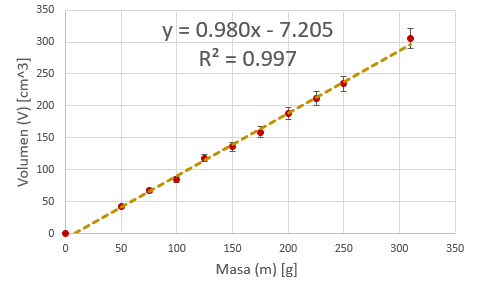
\includegraphics[width=0.8\textwidth]{grafica agua.PNG}
    \captionof{figure}{Gráfica del ajuste por mínimos cuadrados
para los datos del agua linealizados según la
ecuación 2.}
    \label{fig}
\end{Figura}


La densidad resultante para el aceite de soya es:

\begin{equation*}
    m_3 = 0.981 \pm 0.009 \frac{g}{cm^3}
\end{equation*}

y la densidad del aceite de soya es de $0.920 \frac{g}{cm^3}$ $\footnote{http\%3A\%2F\%2Fwww2.inecc.gob.mx\%2Fsistemas\%2Fplaguicidas\%2Fpdf\%2Faceite_de_semilla_de_soya.pdf&clen=17698&chunk=true}$.

\begin{Figura}
\centering
    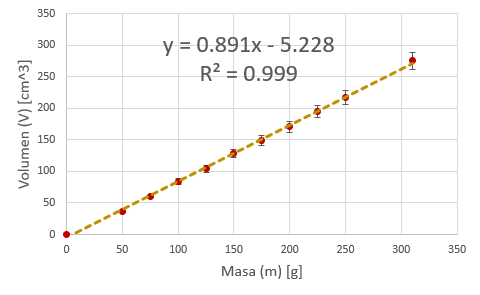
\includegraphics[width=0.8\textwidth]{grafica aceite.PNG}
    \captionof{figure}{Gráfica del ajuste por mínimos cuadrados
para los datos del aceite de soya linealizados según la
ecuación 2.}
    \label{fig}
\end{Figura}


La densidad resultante para el refresco de cola es:

\begin{equation*}
    m_4 = 0.986 \pm 0.014 \frac{g}{cm^3}
\end{equation*}

y la densidad del refresco de cola es de $1.04\frac{g}{cm^3}\footnote{https://cluster-divulgacioncientifica.blogspot.com/2009/05/experimento-de-las-coca-colas.html}$.

\begin{Figura}
\centering
    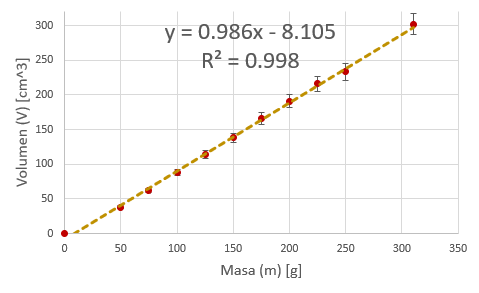
\includegraphics[width=0.8\textwidth]{grafica refresco.PNG}
    \captionof{figure}{Gráfica del ajuste por mínimos cuadrados
para los datos del refresco de cola linealizados según la
ecuación 2.}
    \label{fig}
\end{Figura}


La densidad resultante para el detergente liquido es:

\begin{equation*}
    m_5 = 0.968 \pm 0.011 \frac{g}{cm^3}
\end{equation*}

y la densidad del detergente liquido es de $0.910 \frac{g}{cm^3}\footnote{https://www.contratacion.euskadi.eus/w32-kpeperfi/es/v79aWar/comunJSP/v79aObtenerFichero.do;jsessionid=CWGtz8lGVExYeQWKuolUAA18Y1hxrJBbYXXGKLUZehXL62-GtIcp!444573298!897312586?identificador=860691&idTabla=007&R01HNoPortal=true#:~:text=Densidad\%20al\%2020\%C2\%BAC\%3A\%200\%2C910\%20g\%2Fml.}$.

\begin{Figura}
\centering
    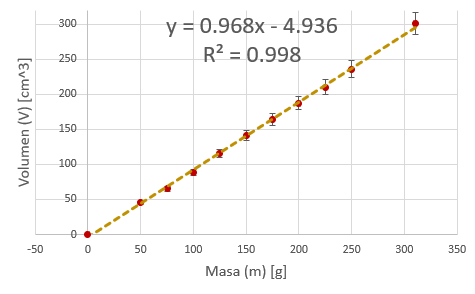
\includegraphics[width=0.8\textwidth]{grafica pinol.PNG}
    \captionof{figure}{Gráfica del ajuste por mínimos cuadrados
para los datos del detergente linealizados según la
ecuación 2.}
    \label{fig}
\end{Figura}


La densidad resultante para el jabón líquido es:

\begin{equation*}
    m_6 = 1.003 \pm 0.008 \frac{g}{cm^3}
\end{equation*}

y la densidad del jabón liquido es $1.028\frac{g}{cm^3}\footnote{chrome-extension://efaidnbmnnnibpcajpcglclefindmkaj/viewer.html?pdfurl=https\%3A\%2F\%2Fwww.javeriana.edu.co\%2Fdocuments\%2F4486808\%2F5015300\%2FJABON\%2BLIQUIDO\%2B_\%2BBIGGEST.pdf\%2F349ce350-524a-4ebb-bcc1-12a6fa6ad1b6\%3Fversion\%3D1.0&pdffilename=JABON\%20LIQUIDO\%20_\%20BIGGEST.pdf}$

\begin{Figura}
\centering
    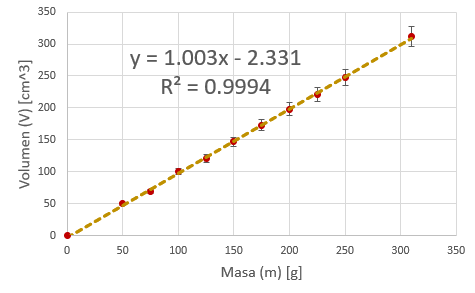
\includegraphics[width=0.8\textwidth]{grafica jabon.PNG}
    \captionof{figure}{Gráfica del ajuste por mínimos cuadrados
para los datos del jabon linealizados según la
ecuación 2.}
    \label{fig}
\end{Figura}






\subsection*{PARTE II}



\begin{Figura}
\centering
    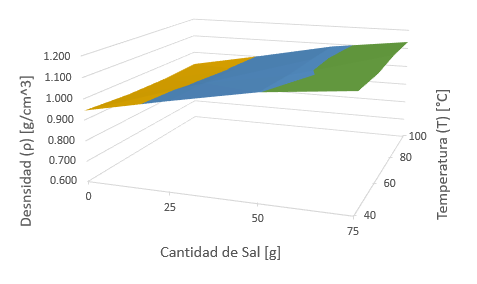
\includegraphics[width=0.8\textwidth]{grafica salinidad 1.PNG}
    \captionof{figure}{Gráfica de la superficie dada por (denisdad vs salinidad vs temperatura) del agua$\footnote{Lamentablemente no encontré la forma de poner incertidumbre a una gráfica de este estilo}$.}
    \label{fig}
\end{Figura}




\begin{Figura}
\centering
    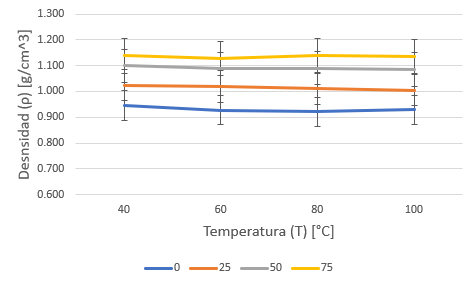
\includegraphics[width=0.8\textwidth]{graficasalinidad 2.PNG}
    \captionof{figure}{Gráfica de cortes de superficie de la gráfica presente en la figura 8.}
    \label{fig}
\end{Figura}

En la figura anterior se puede observar como las gráficas de densidad vs temperatura no parecen cambiar mucho con respecto al aumento de sal, excepto por un desplazamiento hacia arriba conforma aumenta la sal.

\section*{Conclusiones}

\subsection*{PARTE I}
Los intervalos de densidades obtenidas aunque no incluyen los valores reportados, sí se encuentran relativamente cerca por lo que podemos decir que hasta cierto punto corresponden y los resultados son satisfactorios para haberse realizado con material casero.

\subsection*{PARTE II}
Se puede concluir que la densidad del agua aumenta conforme lo hace la cantidad de sal que contiene mientras que para la temperatura no se puede decir mucho.


  
\begin{thebibliography}{99}
\bibitem{1}Halliday, David, Robert Resnick, Kenneth S. Krane, Antonino Pullia, and Lanfranco Cicala. Fisica. Milano: CEA, 2003. 


\bibitem{2} Oda, Berta. Introducción al análisis gráfico de datos experimentales. 3a ed. Ciudad de México: las prensas de ciencias, 2017.



\end{thebibliography}
%\newpage

\section*{Apéndices}

\subsection*{Tablas}



\begin{Figura}
\centering
    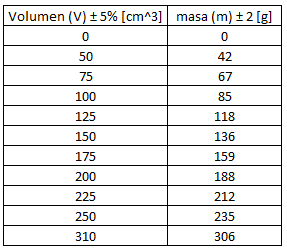
\includegraphics[width=0.8\textwidth]{tabla agua.PNG}
    \captionof{table}{Tabla de volúmenes y masas medidas para el agua.}
    \label{fig}
\end{Figura}


\begin{Figura}
\centering
    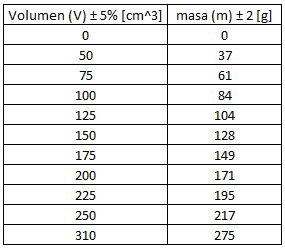
\includegraphics[width=0.8\textwidth]{tabla aceite.PNG}
    \captionof{table}{Tabla de volúmenes y masas medidas para el aceite de Soya (Sabrosano).}
    \label{fig}
\end{Figura}


\begin{Figura}
\centering
    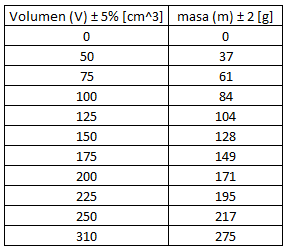
\includegraphics[width=0.8\textwidth]{tabla refresco.PNG}
    \captionof{table}{Tabla de volúmenes y masas medidas para el refresco de cola (Coca Cola).}
    \label{fig}
\end{Figura}



\begin{Figura}
\centering
    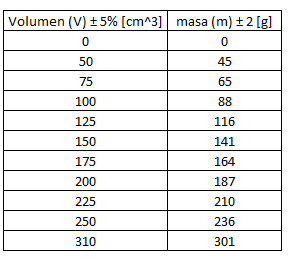
\includegraphics[width=0.8\textwidth]{tabla pinol.PNG}
    \captionof{table}{Tabla de volúmenes y masas medidas para el detergente líquido (Pinol).}
    \label{fig}
\end{Figura}


\begin{Figura}
\centering
    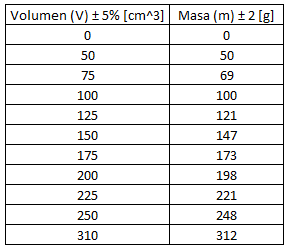
\includegraphics[width=0.8\textwidth]{tabla jabon.PNG}
    \captionof{table}{Tabla de volúmenes y masas medidas para el jabón liquido(Member's Mark).}
    \label{fig}
\end{Figura}

\begin{Figura}
\centering
    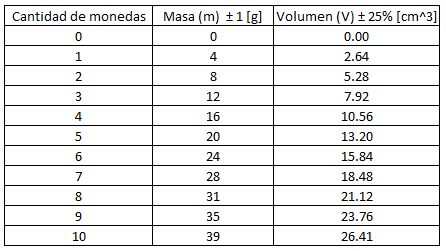
\includegraphics[width=1\textwidth]{tabla monedas.PNG}
    \captionof{table}{Tabla de volúmenes y masas medidas para las monedas de un peso mexicano.}
    \label{fig}
\end{Figura}

PARTE II

\begin{Figura}
\centering
    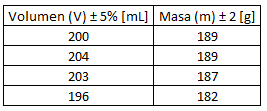
\includegraphics[width=0.8\textwidth]{tabla 0g.PNG}
    \captionof{table}{Tabla de volúmenes y masas medidas del agua para 0 gramos de sal.}
    \label{fig}
\end{Figura}


\begin{Figura}
\centering
    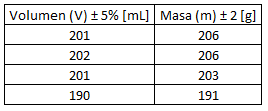
\includegraphics[width=0.8\textwidth]{tabla 25g.PNG}
    \captionof{table}{Tabla de volúmenes y masas medidas del agua para 25 gramos de sal.}
    \label{fig}
\end{Figura}


\begin{Figura}
\centering
    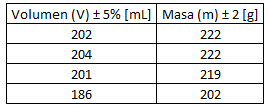
\includegraphics[width=0.8\textwidth]{tabla 50g.PNG}
    \captionof{table}{Tabla de volúmenes y masas medidas del agua para 50 gramos de sal.}
    \label{fig}
\end{Figura}


\begin{Figura}
\centering
    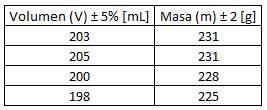
\includegraphics[width=0.8\textwidth]{tabla 75g.PNG}
    \captionof{table}{Tabla de volúmenes y masas medidas del agua para 75 gramos de sal.}
    \label{fig}
\end{Figura}


\end{multicols}
\end{document}